\section{Analysis strategy}
The search targets the $H^+$ production decaying into $tb$ in the single-lepton channel. The events that pass the selection described in Section~\ref{Hplustb:SectionEventSelection} are further divided into two types of disjointed analysis regions: signal regions and control regions. The control regions are used to improve the modelling of the \ttbar+jets background. Furthermore, several multi-variate techniques are used to improve the separation between signal and background events.

\subsection{Region definition}

The analysis regions are categorised as a function of the number of reconstructed jets and $b$-tagged jets at the 70\% $b$-tagging WP. The signal regions are 5j3b, 5j$\geq$4b, $\geq$6j3b and $\geq$6j$\geq$4b. Figure~\ref{Hplustb:cheeseplots} illustrates the background composition, which clearly shows the dominance of the \ttbar\ background, specially the \ttb\ component in the $\geq$4b regions.

\begin{figure}[htbp]
    \RawFloats
    \begin{center}
    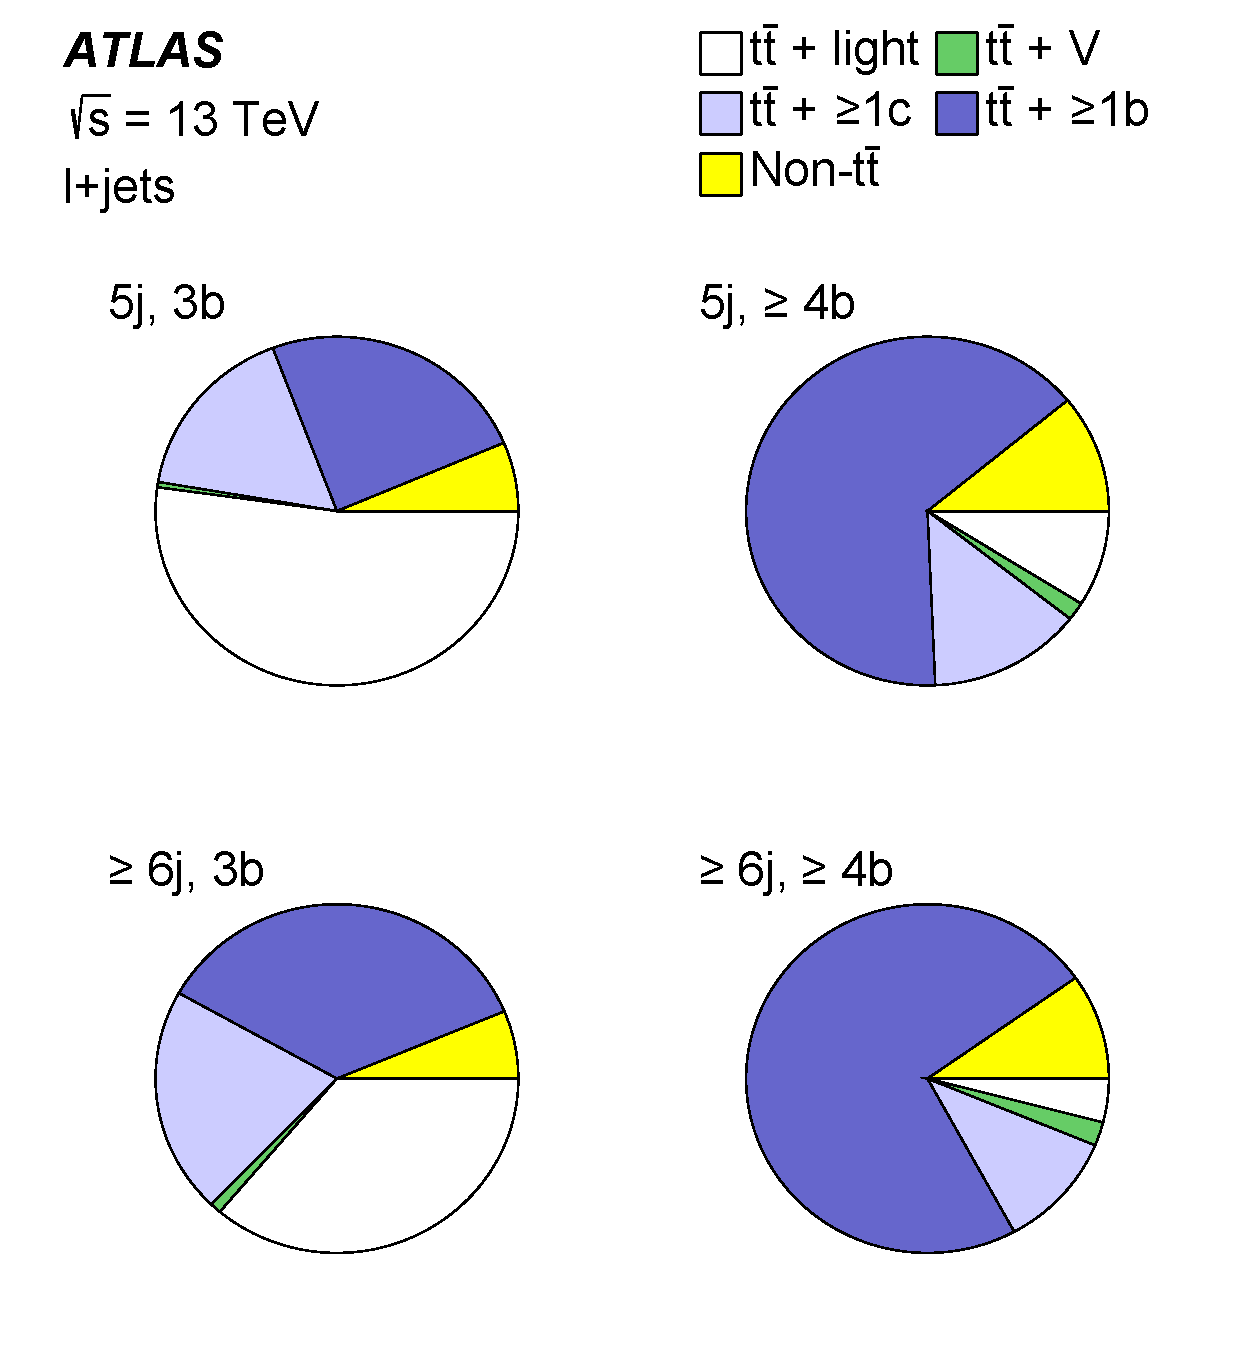
\includegraphics[width=0.5\textwidth]{HPLUSTB/cheeseplot.pdf}
    \caption{
        Background composition in the various analysis regions.
    }
    \label{Hplustb:cheeseplots}
    \end{center}
\end{figure}

Table~\ref{Hplustb:prefityields} shows the number of expected and selected events in the different regions, including the $\geq$5j2b selection which is used to derive weights to improve the background modelling, as shown in the next section. The number of expected $H^+$ signal events for the 600 GeV mass hypothesis is also shown, which is only  contribution is less than 0.5\% for the $\geq$5j2b and thus considered negligible. %Table 6 shows the cut flow for each signal sample.

\begin{table}[htb]
    \centering
    \begin{tabular}{l r r r r r}
        \toprule\toprule
          & $\geq$ 5j, 2b & {5j, 3b} & {5j, $\geq$ 4b} & {$\geq$ 6j, 3b} & {$\geq$ 6j, $\geq$ 4b}\\
          \midrule 
  $t\bar{t}$ + light        & 1365450 $\pm$ 420 & 44000 $\pm$ 8000  & 290 $\pm$ 130  & 31000 $\pm$ 6000  & 340 $\pm$ 180 \\ 
  $t\bar{t}$ + $\geq$1$b$   & 92380   $\pm$ 44 & 20500  $\pm$ 2400  & 2080 $\pm$ 240 & 30000 $\pm$ 4000  & 6100 $\pm$ 1500   \\ 
  $t\bar{t}$ + $\geq$1$c$   & 217830  $\pm$ 120 & 14000 $\pm$ 1600  & 440 $\pm$ 90   & 17800 $\pm$ 2400  & 910  $\pm$ 180   \\ 
  $t\bar{t}$ + $W$          & 3181    $\pm$ 5   & 109   $\pm$ 16    & 3.2 $\pm$ 0.6  & 230   $\pm$ 40    & 15.7   $\pm$ 2.8 \\ 
  $t\bar{t}$ + $Z$          & 3976    $\pm$ 12  & 300   $\pm$ 40    & 51  $\pm$ 7    & 650   $\pm$ 90    & 169  $\pm$ 24 \\ 
  $Wt$ channel              & 46190   $\pm$ 110 & 2300  $\pm$ 600   & 80  $\pm$ 50   & 1800  $\pm$ 800   & 150  $\pm$ 90 \\ 
  $t$ channel               & 19505   $\pm$ 74  & 790   $\pm$ 310   & 55  $\pm$ 21   & 600   $\pm$ 500   & 70   $\pm$ 50 \\ 
  Other top sources         & 1898    $\pm$ 8   & 125   $\pm$ 17    & 17.7  $\pm$ 3.3    & 190   $\pm$ 70    & 60   $\pm$ 24 \\ 
  $VV$ \& $V$ + jets        & 49830   $\pm$ 140 & 1700  $\pm$ 700   & 68  $\pm$ 25   & 1600  $\pm$ 600   & 120  $\pm$ 50 \\ 
  $t\bar{t}H$               & 2918    $\pm$ 2   & 530   $\pm$ 60    & 129 $\pm$ 20   & 1110  $\pm$ 130   & 420  $\pm$ 60 \\ 
\midrule      
  Total                     &1803170 $\pm$ 480 & 84000 $\pm$ 10000 & 3200$\pm$ 400 & 85000 $\pm$ 12000 & 8400 $\pm$ 1700 \\
\midrule
  Data                      &1830756           & 95852             & 4109          & 98929          & 10552 \\
\midrule  
\midrule\ 600 GeV             & 1911 $\pm$ 24   & 520 $\pm$ 40      & 73 $\pm$ 8    & 960 $\pm$ 80   & 279 $\pm$ 25  \\   
\bottomrule\bottomrule                               
    \end{tabular}
    \caption{Number of expected and selected events split according to the analysis regions. The $\geq$ 5j, 2b region is used to derive weights to improve the data/simulation agreement. The quoted uncertainties include both statistical and systematic uncertainties except for the first column ($\geq$ 5j, 2b) which only includes statistical uncertainties. The predicted number of $H^+$ signal events for the 600 GeV mass hypothesis is also shown, assuming a cross-section times branching fraction of 0.32~pb.}
    \label{Hplustb:prefityields}
\end{table}

Figure~\ref{Hplustb:acceptance} shows the acceptance times efficiency of the $\geq$5j$\geq$3b inclusive selection per signal mass sample. It can be observed the decrease in acceptance starting from 1000~GeV due to the loss of jets, characteristic of boosted regimes.

\begin{figure}[htbp]
    \RawFloats
    \begin{center}
    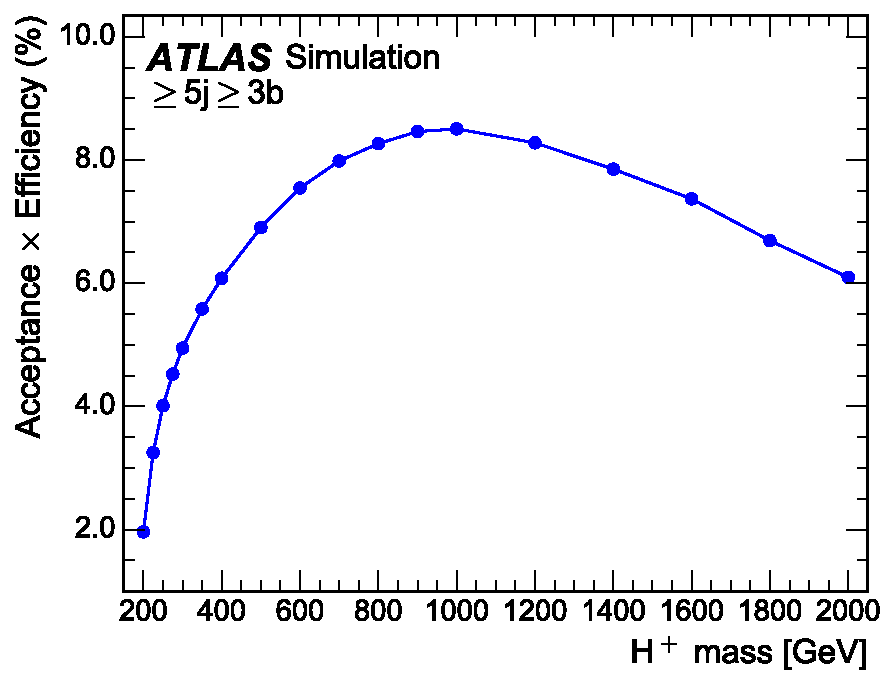
\includegraphics[width=0.5\textwidth]{HPLUSTB/acceptance.pdf}
    \caption{
        Total event acceptance of every $H^+$ signal sample. Statistical uncertainties are included but hidden within the markers.
    }
    \label{Hplustb:acceptance}
    \end{center}
\end{figure}

\clearpage
\subsection{Reweighting technique}

The main background for the search is \ttbar+jets, and its correct modelling is essential for the correct description of the data. It is observed that the simulation does not properly model high jet multiplicities nor the hardness of additional jet emissions %https://cds.cern.ch/record/2630327 https://link.springer.com/article/10.1007/JHEP01(2021)033
To improve the data/MC agreement of this essential background, data-based corrections are applied to the \ttbar samples. Since the mismodelling is assumed to be due mainly to the additional radiation in the parton shower, hence independent on the flavour of the associated jets, the corrections derived in the $\geq$5j2b regions are expected to improve the agreement in the 3b and $\geq$4b regions. The remaining discrepancies can still be covered by the systematic model.

The corrections are derived for each jet multiplicity and as a function of \HTall, defined as the scalar \pT sum of jets and the lepton, i.e. all the selected objects. The reweighting factors for each jet multiplicity is expressed as:

\begin{equation}
    \label{Hplustb:RWeq}
    R(\HTall)=\frac{ Data(\HTall) - \text{MC}^{\text{non-\ttbar}(\HTall)} }{\text{MC}^{\text{\ttbar}(\HTall)}}
\end{equation}

and, by construction, assumes that any disagreement between data and MC is from \ttbar. In this context, \ttbar\ includes \ttb, \ttc\ and \ttl\ as well as single top $tW$ contributions. 

Figure~\ref{Hplustb:RWfactors} includes all the derived corrections, showing higher weights for increased jet multiplicities and, in general, the \HTall corrections have a hyperbolic behaviour: converging $\HTall > 800$~GeV and rapidly increasing towards lower values. Among various functions tried, the hyperbola plus a sigmoid functional form was found to be the best fit to the \HTall weight distributions: $w=a+\frac{b}{(\HTall)^c} - \frac{d}{1+\exp(e-f\cdot\HTall)}$. The eigenvalues of the error matrix of fitted parameters are included as systematic uncertainties. 

\begin{figure}[htb]
    \RawFloats
    \begin{center}
    \subfloat[$\ge$5j2b]{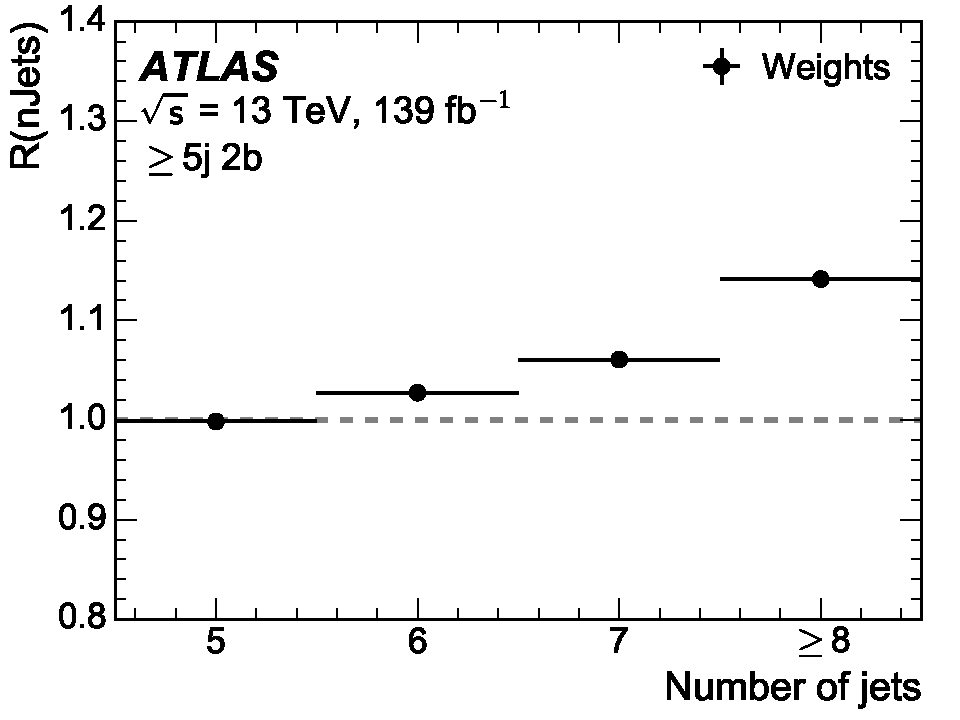
\includegraphics[width = 0.3\textwidth]{HPLUSTB/Reweighting/nominal_jets.pdf}}  
    \subfloat[5j2b]{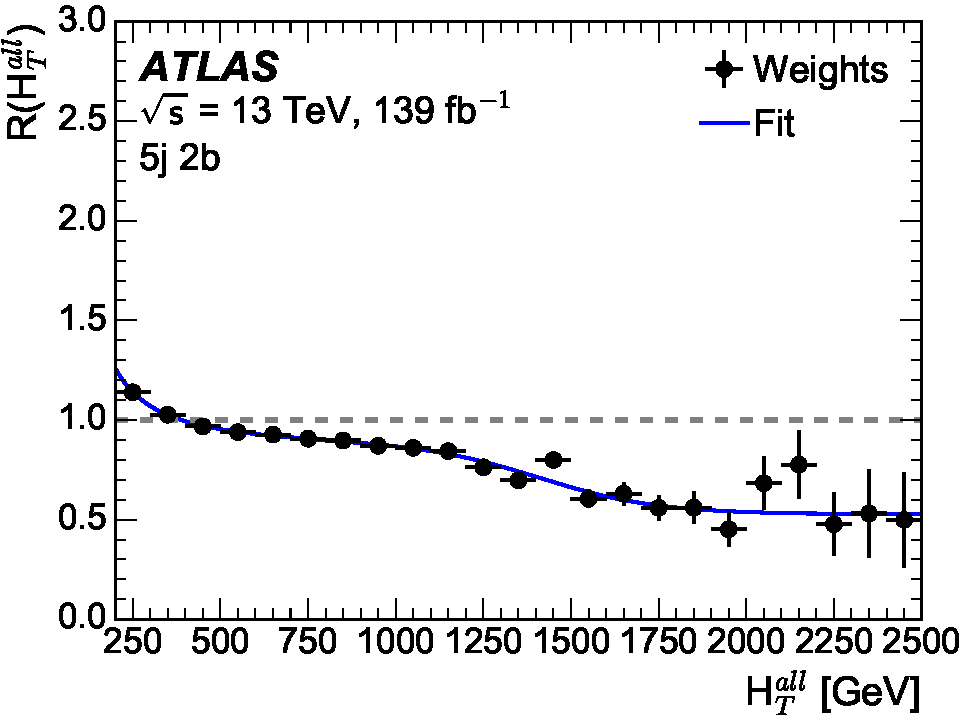
\includegraphics[width = 0.3\textwidth]{HPLUSTB/Reweighting/fitparsvar_hyp_5j.pdf}} 
    \subfloat[6j2b]{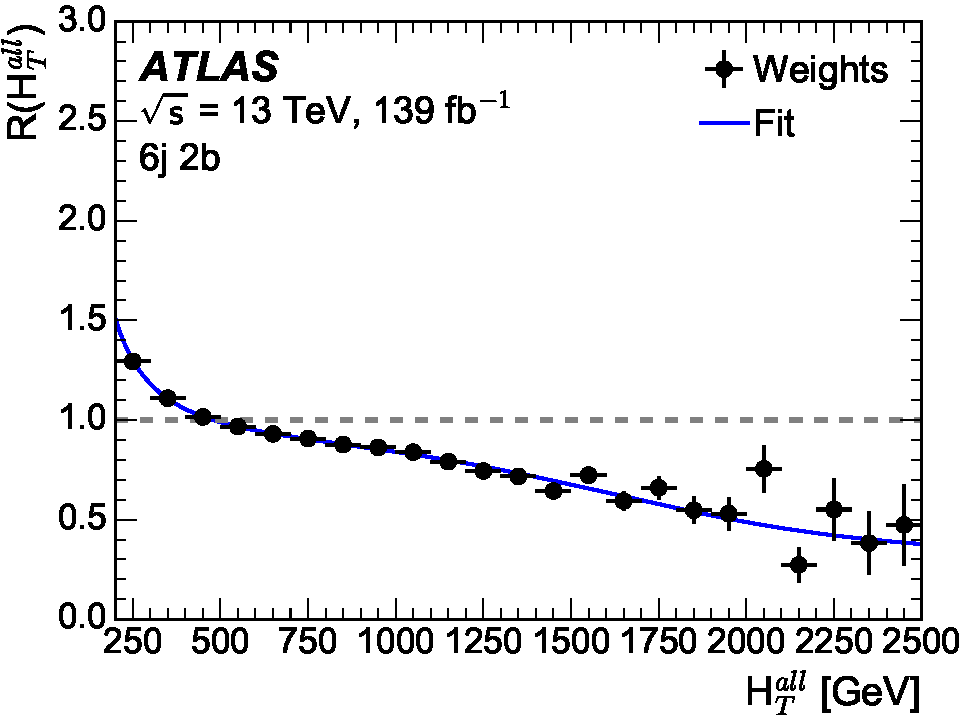
\includegraphics[width = 0.3\textwidth]{HPLUSTB/Reweighting/fitparsvar_hyp_6j.pdf}}  \\
    \subfloat[7j2b]{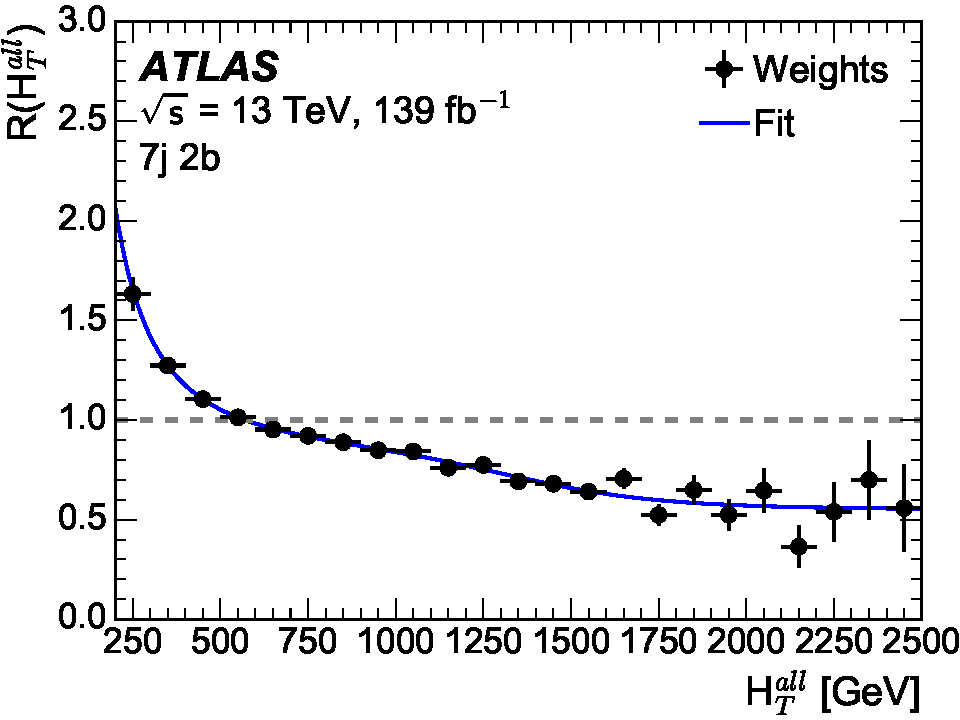
\includegraphics[width = 0.3\textwidth]{HPLUSTB/Reweighting/fitparsvar_hyp_7j.pdf}}
    \subfloat[$\ge$8j2b]{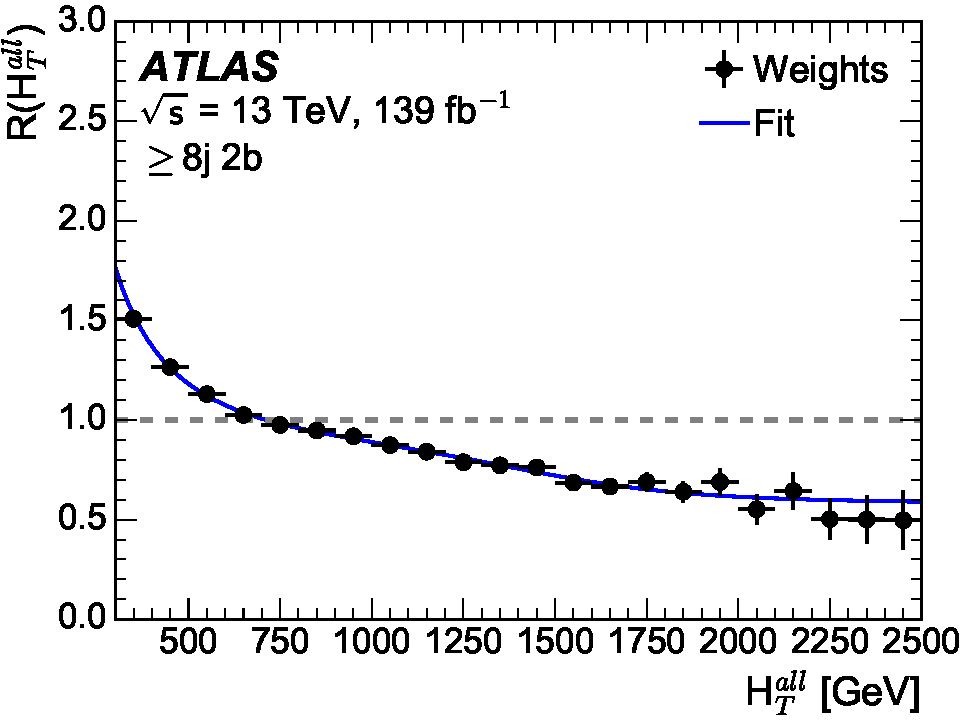
\includegraphics[width = 0.3\textwidth]{HPLUSTB/Reweighting/fitparsvar_hyp_8j.pdf}}
    \caption{Reweighting factors (weights) obtained from the comparison between data and simulation of the number of jets (a) and \HTall\ for various jet multiplicity selections (b) to (e).
    The errors in the data points include the statistical uncertainties in data and MC predictions.}
    \label{Hplustb:RWfactors}
\end{center}
\end{figure}

The agreement between simulation and data in the analysis region improves, as an example, Figure~\ref{Hplustb:RWeffect} shows the improvement in the leading jet \pT\ distribution before and after the reweighting. The remaining disagreement is specially from normalisation effects. All figures included in this document are shown after the reweighting corrections are applied, unless stated otherwise

\begin{figure}[htb]
    \RawFloats
    \begin{center}
    \subfloat[5j3b, unweighted]
    {\includegraphics[width = 0.249\textwidth]{HPLUSTB/Reweighting/unrw/plot_5jex3bex_jet_pt.pdf}}
    \subfloat[5j$\ge$4b, unweighted] 
    {\includegraphics[width = 0.249\textwidth]{HPLUSTB/Reweighting/unrw/plot_5jex4bin_jet_pt.pdf}}
     \subfloat[$\ge$6j3b, unweighted]
    {\includegraphics[width = 0.249\textwidth]{HPLUSTB/Reweighting/unrw/plot_6jin3bex_jet_pt.pdf}}   
     \subfloat[$\ge$6j$\ge$4b, unweighted]
    {\includegraphics[width = 0.249\textwidth]{HPLUSTB/Reweighting/unrw/plot_6jin4bin_jet_pt.pdf}}  \\
     \subfloat[5j3b, reweighted] 
    {\includegraphics[width = 0.249\textwidth]{HPLUSTB/Reweighting/rw/plot_5jex3bex_jet_pt.pdf}} 
     \subfloat[5j$\ge$4b, reweighted] 
    {\includegraphics[width = 0.249\textwidth]{HPLUSTB/Reweighting/rw/plot_5jex4bin_jet_pt.pdf}}    
     \subfloat[$\ge$6j3b, reweighted]
    {\includegraphics[width = 0.249\textwidth]{HPLUSTB/Reweighting/rw/plot_6jin3bex_jet_pt.pdf}} 
     \subfloat[$\ge$6j$\ge$4b, reweighted]
    {\includegraphics[width = 0.249\textwidth]{HPLUSTB/Reweighting/rw/plot_6jin4bin_jet_pt.pdf}} \\  
    \caption{Comparison of the predicted leading jet \pT\ and data before the fit in the four analysis regions before (top) and after (bottom) the reweighting was applied. The uncertainty bands include both the statistical and systematic uncertainties, except for the cross-sections of the \ttb\ and \ttc\ backgrounds.
    The lower panels display the ratio of the data to the total prediction. 
    The hatched bands show the uncertainties before the fit to the data,  which are dominated by systematic uncertainties. The $\chi^2/\mathrm{ndf}$ and the $\chi^2$ probability are also shown. Statistical uncertainties on MC predictions and data are uncorrelated across bins, while systematic uncertainties on the predictions are correlated.}
    \label{Hplustb:RWeffect}
\end{center}
\end{figure}

\subsection{Multivariate techniques}

